\documentclass[aspectratio=169, 12pt]{beamer}

% ─── Theme & Styling ────────────────────────────────────────────────────────
\usetheme{Madrid}
\usecolortheme{default}

\definecolor{iiitmblue}{RGB}{0, 70, 140}
\definecolor{iiitmlight}{RGB}{220, 235, 250}
\definecolor{accentgreen}{RGB}{34, 139, 34}
\definecolor{accentred}{RGB}{180, 30, 30}

\setbeamercolor{palette primary}{bg=iiitmblue, fg=white}
\setbeamercolor{palette secondary}{bg=iiitmblue!80, fg=white}
\setbeamercolor{palette tertiary}{bg=iiitmblue!60, fg=white}
\setbeamercolor{structure}{fg=iiitmblue}
\setbeamercolor{title}{fg=white, bg=iiitmblue}
\setbeamercolor{frametitle}{fg=white, bg=iiitmblue}
\setbeamercolor{block title}{bg=iiitmblue, fg=white}
\setbeamercolor{block body}{bg=iiitmlight, fg=black}
\setbeamercolor{block title alerted}{bg=accentred, fg=white}
\setbeamercolor{block body alerted}{bg=red!5, fg=black}
\setbeamercolor{block title example}{bg=accentgreen, fg=white}
\setbeamercolor{block body example}{bg=green!5, fg=black}
\setbeamercolor{item}{fg=iiitmblue}

\setbeamertemplate{navigation symbols}{}
\setbeamertemplate{footline}{%
  \leavevmode%
  \hbox{%
    \begin{beamercolorbox}[wd=.35\paperwidth,ht=2.5ex,dp=1ex,center]{palette primary}%
      \usebeamerfont{author in head/foot}\insertshortauthor
    \end{beamercolorbox}%
    \begin{beamercolorbox}[wd=.40\paperwidth,ht=2.5ex,dp=1ex,center]{palette secondary}%
      \usebeamerfont{title in head/foot}\insertshorttitle
    \end{beamercolorbox}%
    \begin{beamercolorbox}[wd=.25\paperwidth,ht=2.5ex,dp=1ex,right]{palette tertiary}%
      \usebeamerfont{date in head/foot}%
      \insertframenumber{} / \inserttotalframenumber\hspace*{2ex}
    \end{beamercolorbox}%
  }%
  \vskip0pt%
}

% ─── Packages ────────────────────────────────────────────────────────────────
\usepackage[utf8]{inputenc}
\usepackage[T1]{fontenc}
\usepackage{lmodern}
\usepackage{amsmath}
\usepackage{booktabs}
\usepackage{tikz}
\usepackage{listings}
\usepackage{graphicx}
\usetikzlibrary{shapes.geometric, arrows.meta, positioning, calc}

\lstdefinestyle{beamerstyle}{
    basicstyle=\ttfamily\scriptsize,
    keywordstyle=\color{iiitmblue}\bfseries,
    commentstyle=\color{gray},
    stringstyle=\color{accentgreen},
    backgroundcolor=\color{iiitmlight},
    frame=single,
    rulecolor=\color{iiitmblue!30},
    breaklines=true,
    showstringspaces=false,
    tabsize=2,
}
\lstset{style=beamerstyle}

% ─── Meta ────────────────────────────────────────────────────────────────────
\title[BTP Mid-Term]{Reducing Cross-Node Network Calls in\\Distributed Payment Systems}
\subtitle{B.Tech Project -- Mid-Term Evaluation}
\author[Raman Kapoor]{Raman Kapoor}
\institute[ABV-IIITM]{ABV -- Indian Institute of Information Technology\\and Management, Gwalior\\[0.5em]\textbf{Supervisor:} Dr.\ Rahul Kala}
\date{March 2026}

% ═══════════════════════════════════════════════════════════════════════════
\begin{document}

% ─── Slide 1: Title ─────────────────────────────────────────────────────────
{
\setbeamertemplate{footline}{}
\begin{frame}
\titlepage
\end{frame}
}

% ─── Slide 2: Outline ───────────────────────────────────────────────────────
\begin{frame}{Outline}
\tableofcontents
\end{frame}

% ═══════════════════════════════════════════════════════════════════════════
\section{Problem Statement}
% ═══════════════════════════════════════════════════════════════════════════

% ─── Slide 3: Problem Overview ──────────────────────────────────────────────
\begin{frame}{Problem Statement: Overview}

\begin{block}{Goal}
Reduce redundant cross-node network calls in latency-sensitive distributed payment APIs \textbf{while preserving strict data correctness} required by financial transaction processing.
\end{block}

\vspace{0.4cm}

\begin{columns}[T]
\begin{column}{0.48\textwidth}
\textbf{Context}
\begin{itemize}
    \item Stateless API servers process millions of payment transactions daily
    \item Each request triggers \textbf{5--15 cross-node calls} to Redis/DB
    \item Most fetched data is \textbf{immutable} or \textbf{slowly changing}
\end{itemize}
\end{column}
\begin{column}{0.48\textwidth}
\textbf{Key Challenges}
\begin{itemize}
    \item Correctness is \textbf{non-negotiable} in payments
    \item Stale data $\Rightarrow$ wrong routing, failed settlements
    \item p95 tail latency spikes under load
    \item Redis load amplification at peak
\end{itemize}
\end{column}
\end{columns}

\end{frame}

% ─── Slide 4: The Latency Problem ──────────────────────────────────────────
\begin{frame}{The Latency Problem}

\begin{columns}[T]
\begin{column}{0.55\textwidth}
\textbf{Request Lifecycle (5--15 network calls):}
\begin{enumerate}
    \item Session/Auth lookup $\rightarrow$ Redis
    \item Merchant config $\rightarrow$ Redis/DB
    \item Gateway routing tables $\rightarrow$ Redis
    \item Risk/compliance rules $\rightarrow$ Redis
    \item Rate-limit counters $\rightarrow$ Redis
    \item Transaction processing $\rightarrow$ Gateway
\end{enumerate}

\vspace{0.3cm}
Steps 2--4 involve data that is \textbf{overwhelmingly immutable} within seconds to minutes.
\end{column}

\begin{column}{0.42\textwidth}
\textbf{Baseline Performance:}
\vspace{0.2cm}

\begin{tabular}{@{} l r @{}}
\toprule
\textbf{Metric} & \textbf{Value} \\
\midrule
Peak RPS/node & 2--5K \\
Calls/request & 5--15 \\
Redis RTT & 0.5--2\,ms \\
p50 latency & $\sim$20\,ms \\
p95 latency & $\sim$100\,ms \\
p99 latency & $\sim$300\,ms \\
\bottomrule
\end{tabular}

\vspace{0.3cm}
\textcolor{accentred}{\textbf{Gap between p50 and p95 is driven by network variability.}}
\end{column}
\end{columns}

\end{frame}

% ═══════════════════════════════════════════════════════════════════════════
\section{Data Classification}
% ═══════════════════════════════════════════════════════════════════════════

% ─── Slide 5: Data Classification ──────────────────────────────────────────
\begin{frame}{Data Classification: What Can Be Cached?}

\begin{center}
\small
\begin{tabular}{@{} l l l c @{}}
\toprule
\textbf{Data Category} & \textbf{Mutation Freq.} & \textbf{Scope} & \textbf{Cache-Safe?} \\
\midrule
Merchant Configuration & Daily or less & Global & \textcolor{accentgreen}{\textbf{Yes}} \\
Gateway Routing Tables & Weekly or less & Global & \textcolor{accentgreen}{\textbf{Yes}} \\
Feature Flags & Hourly or less & Global & \textcolor{accentgreen}{\textbf{Yes}} \\
Compliance Rules & Quarterly & Global & \textcolor{accentgreen}{\textbf{Yes}} \\
\midrule
Rate Limit Counters & Per-request & Per-user & \textcolor{accentred}{\textbf{No}} \\
Idempotency Records & Per-request & Per-txn & \textcolor{accentred}{\textbf{No}} \\
Transaction State & Per-request & Per-txn & \textcolor{accentred}{\textbf{No}} \\
Session/Auth Tokens & Per-session & Per-user & \textcolor{accentred}{\textbf{No}} \\
\bottomrule
\end{tabular}
\end{center}

\vspace{0.3cm}

\begin{alertblock}{Key Insight}
The first 4 categories represent the \textbf{majority of cross-node lookups by volume} and are candidates for safe caching. Classification is \textbf{binary} -- no ``partially safe'' category.
\end{alertblock}

\end{frame}

% ═══════════════════════════════════════════════════════════════════════════
\section{Proposed Approach}
% ═══════════════════════════════════════════════════════════════════════════

% ─── Slide 6: Two-Tier Caching Overview ────────────────────────────────────
\begin{frame}{Proposed Approach: Two-Tier Caching}

\begin{center}
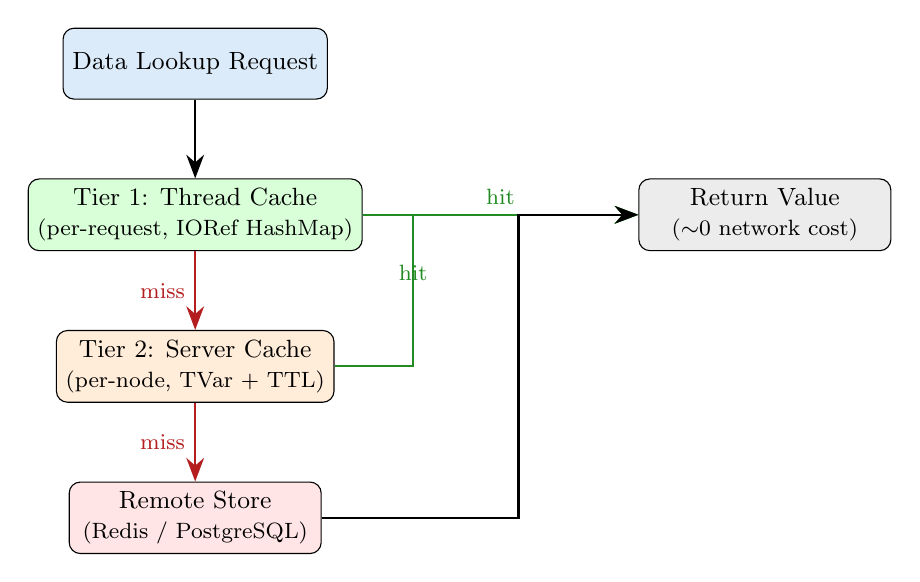
\begin{tikzpicture}[
    box/.style={rectangle, draw, rounded corners, minimum width=3.2cm, minimum height=0.9cm, align=center, font=\small},
    arrow/.style={-{Stealth[length=3mm]}, thick},
    yes/.style={font=\footnotesize, accentgreen},
    no/.style={font=\footnotesize, accentred},
    node distance=1.3cm
]
    \node[box, fill=iiitmlight] (lookup) {Data Lookup Request};
    \node[box, fill=green!15, below=1cm of lookup] (t1) {Tier 1: Thread Cache\\{\footnotesize (per-request, IORef HashMap)}};
    \node[box, fill=orange!15, below=1cm of t1] (t2) {Tier 2: Server Cache\\{\footnotesize (per-node, TVar + TTL)}};
    \node[box, fill=red!10, below=1cm of t2] (remote) {Remote Store\\{\footnotesize (Redis / PostgreSQL)}};
    \node[box, fill=gray!15, right=3.5cm of t1] (ret) {Return Value\\{\footnotesize ($\sim$0 network cost)}};

    \draw[arrow] (lookup) -- (t1);
    \draw[arrow, accentgreen] (t1) -- node[above, yes] {hit} (ret);
    \draw[arrow, accentred] (t1) -- node[left, no] {miss} (t2);
    \draw[arrow, accentgreen] (t2.east) -- ++(1,0) |- node[near start, above, yes] {hit} (ret);
    \draw[arrow, accentred] (t2) -- node[left, no] {miss} (remote);
    \draw[arrow] (remote.east) -- ++(2.5,0) |- (ret);
\end{tikzpicture}
\end{center}

\vspace{0.2cm}
\textbf{Key property:} Entirely in-process. \textbf{Zero additional infrastructure.}

\end{frame}

% ─── Slide 7: Tier 1 — Thread-Level Cache ──────────────────────────────────
\begin{frame}{Tier 1: Thread-Level Cache (Request-Scoped)}

\begin{columns}[T]
\begin{column}{0.55\textwidth}
\textbf{Design:}
\begin{itemize}
    \item Created when a request arrives
    \item \texttt{IORef (HashMap Text ByteString)}
    \item First fetch $\rightarrow$ store in cache
    \item Subsequent lookups $\rightarrow$ cache hit
    \item Destroyed when request completes
\end{itemize}

\vspace{0.3cm}
\textbf{Why it works:}
\begin{itemize}
    \item A single request fetches the \textbf{same merchant config 2--4 times} (auth, routing, fees)
    \item Thread cache deduplicates these
\end{itemize}
\end{column}

\begin{column}{0.42\textwidth}
\begin{exampleblock}{Correctness Guarantee}
\textbf{Strongest possible:} cache lives only for the request lifetime $\Rightarrow$ impossible for data to become stale.
\end{exampleblock}

\vspace{0.3cm}
\begin{block}{Expected Impact}
Eliminates \textbf{2--4 redundant} network calls per request out of 5--15 total.
\end{block}
\end{column}
\end{columns}

\end{frame}

% ─── Slide 8: Tier 2 — Server-Local Cache ──────────────────────────────────
\begin{frame}{Tier 2: Server-Local Cache (Node-Scoped)}

\begin{columns}[T]
\begin{column}{0.55\textwidth}
\textbf{Design:}
\begin{itemize}
    \item Shared across all threads on a node
    \item Concurrent \texttt{TVar}-based HashMap
    \item \textbf{Short TTL:} 30--60 seconds
    \item Bounded size + LRU eviction
    \item Background eviction thread
\end{itemize}

\vspace{0.3cm}
\textbf{Motivation:}\\
1,000 RPS on one node, all fetching same merchant config $\Rightarrow$ 999 redundant calls. Server cache serves from memory after the first.
\end{column}

\begin{column}{0.42\textwidth}
\textbf{TTL Rationale:}
\vspace{0.2cm}

\begin{tabular}{@{} l r @{}}
\toprule
\textbf{Data} & \textbf{TTL} \\
\midrule
Merchant cfg & 30\,s \\
Routes & 60\,s \\
Feature flags & 30\,s \\
\bottomrule
\end{tabular}

\vspace{0.4cm}
\begin{alertblock}{Staleness Impact}
Worst case: config change takes effect 30\,s later. \textbf{No financial impact.}
\end{alertblock}
\end{column}
\end{columns}

\end{frame}

% ═══════════════════════════════════════════════════════════════════════════
\section{Cache-Safety Boundaries}
% ═══════════════════════════════════════════════════════════════════════════

% ─── Slide 9: Cache-Safety Criteria ────────────────────────────────────────
\begin{frame}{Cache-Safety Boundaries: Formal Criteria}

A data item $d$ is \textbf{cache-safe} if and only if \textbf{all four} conditions hold:

\vspace{0.3cm}

\begin{enumerate}
    \item \textbf{Immutability within TTL:} $d(t) = d(t')$ for all $t' \in [t,\, t + \Delta]$

    \item \textbf{Request-Scope Independence:} $d$ depends only on global/slow-changing state, not on request-specific parameters

    \item \textbf{Semantic Idempotency of Stale Reads:} Even if $d$ is briefly stale, the system produces a \textbf{semantically correct} outcome

    \item \textbf{Deterministic Cache Key:} Key is deterministically derivable from lookup parameters (no collisions)
\end{enumerate}

\vspace{0.3cm}

\begin{block}{Design Philosophy}
Classification is \textbf{binary}. No ``partially safe'' category.  If \textbf{any} criterion fails $\Rightarrow$ data is \textbf{not cached}.
\end{block}

\end{frame}

% ═══════════════════════════════════════════════════════════════════════════
\section{Implementation}
% ═══════════════════════════════════════════════════════════════════════════

% ─── Slide 10: Implementation ──────────────────────────────────────────────
\begin{frame}[fragile]{Implementation: Haskell/GHC Runtime}

\begin{columns}[T]
\begin{column}{0.48\textwidth}
\textbf{Thread-Level Cache:}
\begin{lstlisting}[language=Haskell]
type ThreadCache =
  IORef (HashMap Text ByteString)

cachedLookup :: ThreadCache
             -> Text -> IO ByteString
             -> IO ByteString
cachedLookup ref key fetch = do
  cache <- readIORef ref
  case HM.lookup key cache of
    Just v  -> return v
    Nothing -> do
      v <- fetch
      modifyIORef' ref (HM.insert key v)
      return v
\end{lstlisting}
\end{column}

\begin{column}{0.48\textwidth}
\textbf{Server-Local Cache:}
\begin{lstlisting}[language=Haskell]
data CacheEntry = CacheEntry
  { ceValue     :: !ByteString
  , ceExpiresAt :: !Double }

type ServerCache =
  TVar (HashMap Text CacheEntry)

-- TTL check via STM
-- Background eviction thread
-- runs every 10 seconds
\end{lstlisting}

\vspace{0.2cm}
\textbf{Cache Key Design:}
\begin{lstlisting}[language=Haskell]
"mc:" <> merchantId  -- config
"gr:" <> gatewayId   -- routes
"ff:" <> flagName    -- flags
\end{lstlisting}
\end{column}
\end{columns}

\end{frame}

% ═══════════════════════════════════════════════════════════════════════════
\section{Evaluation \& Results}
% ═══════════════════════════════════════════════════════════════════════════

% ─── Slide 11: Methodology ─────────────────────────────────────────────────
\begin{frame}{Evaluation: Methodology}

Deployed via \textbf{staged rollout} on the production platform:

\vspace{0.3cm}

\begin{enumerate}
    \item \textbf{Baseline Measurement} -- 1-week metrics without caching
    \item \textbf{Canary Deployment} -- caching on subset of nodes (canary group)
    \item \textbf{Full Rollout} -- enabled across all nodes after validation
    \item \textbf{Post-Rollout Observation} -- extended monitoring for correctness
\end{enumerate}

\vspace{0.5cm}

\begin{exampleblock}{Production Scale}
\textbf{$\sim$68,000 cross-node operations/sec} at peak traffic across all API server nodes.
\end{exampleblock}

\end{frame}

% ─── Slide 12: Key Results ─────────────────────────────────────────────────
\begin{frame}{Results: Network Call \& Latency Reduction}

\begin{columns}[T]
\begin{column}{0.48\textwidth}
\textbf{Cross-Node Call Reduction:}
\vspace{0.2cm}

\small
\begin{tabular}{@{} l r r @{}}
\toprule
\textbf{Metric} & \textbf{Before} & \textbf{After} \\
\midrule
Calls/request & 10.2 & 8.7 \\
Peak ops/sec & 68,400 & 65,600 \\
Thread-cache hit & -- & 22.3\% \\
Server-cache hit & -- & 41.7\% \\
\textbf{Combined hit} & -- & \textbf{54.8\%} \\
\bottomrule
\end{tabular}
\normalsize

\vspace{0.3cm}
\textcolor{iiitmblue}{\textbf{4.1\% reduction at peak}} = $\sim$2,800 fewer network calls \textit{per second.}
\end{column}

\begin{column}{0.48\textwidth}
\textbf{Latency Improvement:}
\vspace{0.2cm}

\small
\begin{tabular}{@{} l r r r @{}}
\toprule
\textbf{Pctl} & \textbf{Before} & \textbf{After} & \textbf{$\Delta$} \\
\midrule
p50 & 22\,ms & 20\,ms & $-$9\% \\
\textbf{p95} & \textbf{98\,ms} & \textbf{87\,ms} & $-$\textbf{11\%} \\
p99 & 285\,ms & 248\,ms & $-$13\% \\
\bottomrule
\end{tabular}
\normalsize

\vspace{0.3cm}

\textbf{Redis p99 latency:}\\
4.2\,ms $\rightarrow$ 3.1\,ms (\textcolor{accentgreen}{\textbf{$-$26.2\%}})

\vspace{0.1cm}
{\small Virtuous cycle: less load $\Rightarrow$ faster Redis $\Rightarrow$ faster APIs.}
\end{column}
\end{columns}

\end{frame}

% ─── Slide 13: Correctness ─────────────────────────────────────────────────
\begin{frame}{Results: Correctness \& Overhead}

\begin{columns}[T]
\begin{column}{0.48\textwidth}
\begin{block}{Correctness Validation}
Over the observation period:
\begin{itemize}
    \item \textcolor{accentgreen}{\textbf{Zero}} cache-related incidents
    \item \textcolor{accentgreen}{\textbf{Zero}} financial discrepancies
    \item \textcolor{accentgreen}{\textbf{Zero}} compliance violations
    \item All mutable/transactional data bypasses cache entirely
\end{itemize}
\end{block}
\end{column}

\begin{column}{0.48\textwidth}
\begin{block}{Memory Overhead}
\vspace{0.2cm}
\begin{tabular}{@{} l r @{}}
\toprule
\textbf{Component} & \textbf{Memory} \\
\midrule
Thread cache/req & 2--10\,KB \\
Server cache/node & 5--15\,MB \\
\textbf{Total/node} & $<$\textbf{20\,MB} \\
\bottomrule
\end{tabular}
\vspace{0.2cm}
\end{block}

\vspace{0.2cm}
\begin{exampleblock}{Implementation Cost}
$\sim$\textbf{200--300 lines} of code.\\
Localised to caching module.\\
Business logic \textbf{unchanged}.
\end{exampleblock}
\end{column}
\end{columns}

\end{frame}

% ═══════════════════════════════════════════════════════════════════════════
\section{Discussion}
% ═══════════════════════════════════════════════════════════════════════════

% ─── Slide 14: Why 4% Matters ──────────────────────────────────────────────
\begin{frame}{Discussion: Why 4\% Matters at Scale}

\begin{columns}[T]
\begin{column}{0.48\textwidth}
\textbf{Scale amplifies small percentages:}
\begin{itemize}
    \item 68,000 ops/sec $\times$ 4\% = \textbf{2,800 fewer calls/sec}
    \item Over 24 hours $\approx$ \textbf{240 million fewer calls}
    \item Each avoided call saves RTT, CPU (ser/deser), bandwidth
    \item \textbf{Second-order:} less Redis load $\Rightarrow$ lower Redis latency $\Rightarrow$ faster APIs
\end{itemize}

\vspace{0.2cm}
Off-peak reduction is even higher: \textbf{7--10\%}.
\end{column}

\begin{column}{0.48\textwidth}
\textbf{Comparison with alternatives:}
\vspace{0.2cm}

\small
\begin{tabular}{@{} l c c @{}}
\toprule
\textbf{Approach} & \textbf{Infra} & \textbf{Risk} \\
\midrule
Redis replica & High & Low \\
CDN for APIs & Med & High \\
DB replicas & High & Med \\
\textbf{Our approach} & \textbf{None} & \textbf{None} \\
\bottomrule
\end{tabular}
\normalsize

\vspace{0.3cm}
\begin{block}{Unique Position}
\textbf{Zero-cost, zero-risk} optimisation by construction.
\end{block}
\end{column}
\end{columns}

\end{frame}

% ═══════════════════════════════════════════════════════════════════════════
\section{Future Work}
% ═══════════════════════════════════════════════════════════════════════════

% ─── Slide 15: Future Work ─────────────────────────────────────────────────
\begin{frame}{Future Work}

\begin{enumerate}
    \item \textbf{Adaptive TTL Management}\\
    {\small Monitor mutation frequency per data class; dynamically adjust TTLs to maximise hit rates while respecting staleness constraints.}

    \vspace{0.3cm}
    \item \textbf{Cache-Aware Load Balancing}\\
    {\small Route all requests for a given merchant to the same node $\Rightarrow$ higher cache hit rates. Balance with load distribution uniformity.}

    \vspace{0.3cm}
    \item \textbf{Pub/Sub-Based Invalidation}\\
    {\small Extend server-local cache to higher-mutation data classes with active invalidation, reducing worst-case staleness to near-zero.}

    \vspace{0.3cm}
    \item \textbf{Type-Level Safety Verification}\\
    {\small Formalise cache-safety criteria as Haskell type-level constraints for compile-time verification.}
\end{enumerate}

\end{frame}

% ═══════════════════════════════════════════════════════════════════════════
\section{Internship Work Highlights}
% ═══════════════════════════════════════════════════════════════════════════

% ─── Slide 16: Internship 1 ────────────────────────────────────────────────
\begin{frame}{Internship: High-Performance Block Storage}

\begin{block}{Lightbits Labs NVMe/TCP Deployment}
Evaluated and deployed Lightbits NVMe-over-TCP as a high-performance alternative to traditional Ceph block storage for database workloads.
\end{block}

\vspace{0.3cm}

\begin{columns}[T]
\begin{column}{0.48\textwidth}
\textbf{The Ceph Problem:}
\begin{itemize}
    \item High hardware footprint (up to 30\% of nodes)
    \item Performance degrades at scale
    \item High tuning complexity (CRUSH, PGs)
\end{itemize}
\end{column}

\begin{column}{0.48\textwidth}
\textbf{The Lightbits Solution:}
\begin{itemize}
    \item Standard TCP network (No RDMA)
    \item Dense NVMe scaling $\Rightarrow$ 10$\times$ hardware footprint reduction
    \item Up to 10M IOPS predictability
    \item OpenStack Cinder integration
\end{itemize}
\end{column}
\end{columns}

\end{frame}

% ─── Slide 17: Internship 2 ────────────────────────────────────────────────
\begin{frame}{Internship: HSM-Backed Key Management}

\begin{block}{OpenStack Barbican \& HSM Integration}
Integrated an external Hardware Security Module (HSM) with OpenStack Barbican to establish a cryptographically secure, multi-tenant secret management pipeline.
\end{block}

\vspace{0.3cm}

\textbf{Security Architecture:}
\begin{itemize}
    \item \textbf{Envelope Encryption:} Secrets encrypted via software; Master Key Wrapping (KEK) done strictly inside the FIPS 140-2 Level 3 HSM hardware.
    \item \textbf{Per-Tenant Isolation:} Unique KEKs generated for each project tenant.
    \item \textbf{Defence in Depth:} Database compromise yields only encrypted payloads and wrapped metadata; unusable without HSM access.
    \item \textbf{Audit \& Compliance:} Satisfies PCI-DSS, HIPAA, and SOC 2 requirements.
\end{itemize}

\end{frame}

% ─── Slide 18: Internship 3 ────────────────────────────────────────────────
\begin{frame}{Internship: Distributed Payout Scheduling}

\begin{block}{Event-Driven Payout System}
Designed and implemented a distributed, event-driven payout scheduling microservice for a ride-hailing platform (10,000+ daily rides).
\end{block}

\vspace{0.3cm}

\begin{columns}[T]
\begin{column}{0.55\textwidth}
\textbf{Architecture \& Flow:}
\begin{enumerate}
    \item Ride completion fires a Kafka event
    \item Payment gateway (Paytm EDC) triggered
    \item Status polling scheduled via Redis Sorted Sets (\texttt{ZADD})
    \item Exponential backoff on polling (max 5 retries)
    \item Idempotent state machine to prevent double-payouts
\end{enumerate}
\end{column}

\begin{column}{0.42\textwidth}
\textbf{Business Impact:}
\vspace{0.2cm}

\begin{itemize}
    \item \textbf{Latency:} Reduced from weekly batch cycles to \textbf{T+2 hours}
    \item \textbf{Scale:} O(1) scheduling throughput
    \item \textbf{Reliability:} Zero impact on ride-booking latency
\end{itemize}
\end{column}
\end{columns}

\end{frame}

% ═══════════════════════════════════════════════════════════════════════════
\section{Summary}
% ═══════════════════════════════════════════════════════════════════════════

% ─── Slide 19: Summary ─────────────────────────────────────────────────────
\begin{frame}{Summary}

\begin{enumerate}
    \item \textbf{Thread-level cache} eliminates intra-request redundancy $\Rightarrow$ 22.3\% hit rate, saves 2--4 calls/request.

    \vspace{0.2cm}
    \item \textbf{Server-local cache} eliminates inter-request redundancy $\Rightarrow$ 41.7\% hit rate, \textbf{4.1\% peak call reduction}.

    \vspace{0.2cm}
    \item \textbf{Combined:} p95 latency $-$11.2\%, p99 latency $-$13.0\%, \textbf{zero correctness violations}.

    \vspace{0.2cm}
    \item \textbf{Cache-safety boundaries} provide rigorous binary classification $\Rightarrow$ correctness by construction.

    \vspace{0.2cm}
    \item \textbf{Minimal cost:} $\sim$200--300 LoC, $<$20\,MB memory/node, zero new infrastructure.
\end{enumerate}

\vspace{0.3cm}

\begin{block}{Key Takeaway}
A lightweight, in-process caching strategy with formal safety guarantees can deliver measurable latency improvements in correctness-critical distributed payment systems \textbf{without any infrastructure changes}.
\end{block}

\end{frame}

% ─── Slide 20: Thank You ──────────────────────────────────────────────────
{
\setbeamertemplate{footline}{}
\begin{frame}
\centering
\vspace{2cm}
{\Huge\bfseries\textcolor{iiitmblue}{Thank You}}\\[1cm]
{\Large Questions?}\\[1.5cm]
{\large Raman Kapoor}\\[0.3cm]
% Enrollment No.: XXXX-XXX\\[0.2cm]
{\normalsize ABV-IIITM Gwalior}
\end{frame}
}

\end{document}
